%\documentclass[12pt,a4paper]{article}
\documentclass[letterpaper,12pt,titlepage]{article}

\usepackage{hyperref}
\usepackage{listings}
\usepackage{wasysym}
\usepackage{graphicx}


\hypersetup{
	colorlinks,
	citecolor=black,
	filecolor=black,
	linkcolor=black,
	urlcolor=black
}

% This is a comment
\title{User Stories and Set-up Assignment}
\author{
  \texttt{Sarahi Pelayo (pelayos)}
  \\[.5ex]
  \texttt{Katherine Jeffrey (jeffreyk)}
  \\[.5ex]
  \texttt{Megan Bigelow (bigelowm)}
  \\[.5ex]
  \texttt{Johnathan Lee (leejohna)}
  \\[.5ex]
  \texttt{Jonathan Rohr (rohrj)}
}

\begin{document}
\maketitle

\section{Stories}
\begin{enumerate}
%1
\item Make emergency call 1:
\newline
The user wants to call poison control quickly from the home page.
%2
\item Make emergency call 2:
\newline
The user wants to call 911 quickly from the home page.
%3
\item Make emergency call 3:
\newline
The user wants to call the suicide hotline quickly from the home page.
%4
\item Setting up for privacy:
\newline
A tutorial shows the user how to set a passcode of their choice.
%4
\item Security feature works:
\newline
The app only opens for that pin and the user receives message that incorrect pin was entered so they know to try again.
%6
\item Change in security feature:
\newline
The user wants to change their passcode to something different and the old passcode will not open the app after the change.(optional)
%7
\item Use of information page part 1:
\newline
The user wants to learn about statistics on PTSD.
%8
\item Use of information page part 2:
\newline
The user want to learn about symptoms of depression.
%9
\item Use of information page part 3:
\newline
The user wants to learn about different definitions related to sexual assault.
%10
\item Use of information page part 4:
\newline
The user wants to visit an external website that is listed under the information to verify or to learn more.
%11
\item Log for today:
\newline
The user wants to input their symptoms on today’s date.
%12
\item Log previous:
\newline
The user wants to input symptoms on a previous date.
%13
\item Log at previous logs:
\newline
The user wants to look at symptoms logged on previous dates.
%14
\item Use resources part 1:
\newline
The user wants to call a sexual assault helpline found in resources page.
%15
\item Use resources part 2:
\newline
The user wants to call a psychiatric help line found in the resources page to find professional help.
%16
\item Use resources part 3:
\newline
The user wants to visit an external website located in the resources page.
%17
\item Use resources part 4:
\newline
The user wants to be sure that the listed addresses will be up to date and correct when they visit them. 
%18
\item Search information and resources:
\newline
The user wants to search the info and resources pages for a specific word or phrase (optional).
\end{enumerate}


\newpage
\section{Tasks (10-20)}
Implement Calling:
\newline
Due Date: 3/15/2018
\newline
Assigned team members: Megan
\newline
Implementation Difficulty(1-10): 6
\newline
Estimated Effort: 3u
\begin{itemize}
\item Access phone calling with application permissions (complete before last step)
\item List phone numbers so user can click (complete before last step)
\item On click, call number
\end{itemize}
Being able to dial from the application to a phone number is used by both the home page emergency number and the resources page with many other useful numbers. Completing this task will be useful for stories 1,2,3,14, and 15.
\newline
\newline
Implement launching an external website:
\newline
Due Date: 3/12/2018 
\newline
Assigned team members: Jonathan Rohr and Johnathan Lee
\newline
Implementation Difficulty(1-10): 5
\newline
Estimated Effort: .5u
\begin{itemize}
\item Access website with application permissions (complete before last step)
\item List link so user can click (complete before last step)
\item On click, visit website
\end{itemize}
Being able to launch an external website from the application then visiting it will be used both by the information pages and the resources pages. Completing this task will add functionality that will be useful for stories 10, and 16.
\newline
\newline
Implement passcode check:
\newline
Due Date: 3/5/2018
\newline
Assigned team members: Sarahi
\newline
Implementation Difficulty(1-10): 6
\newline
Estimated Effort: 2u
\begin{itemize}
\item With incorrect pin, give error message
\item With correct pin, open app
\end{itemize}
Completing this task with give functionality to story number 5.
\newline
\newline
Implement start tutorial (optional):
\newline
Due Date: (optional)
\newline
Assigned team members: (optional)
\newline
Implementation Difficulty(1-10): 7
\newline
Estimated Effort: 5u
\begin{itemize}
\item Guide user through first time install
\item Show user how to find information
\end{itemize}
Completing this task with give functionality to story number 4.
\newline
\newline
Implement change passcode (optional): 
\newline
Due Date: (optional)
\newline
Assigned team members: (optional)
\newline
Implementation Difficulty(1-10): 6
\newline
Estimated Effort: 5u
\begin{itemize}
\item Allow user to change passcode in the settings page.
\end{itemize}
Completing this task with give functionality to story number 6.
\newline
\newline
Implement log current
\newline
Due Date: 3/5/2018
\newline
Assigned team members: Katherine
\newline
Implementation Difficulty(1-10): 10
\newline
Estimated Effort: 10u
\begin{itemize}
\item User can add symptoms for the current day
\end{itemize}
Completing this task with give functionality to story number 11.
\newline
\newline
Implement log previous
\newline
Due Date: 3/12/2018
\newline
Assigned team members: Katherine
\newline
Implementation Difficulty(1-10): 4
\newline
Estimated Effort: 3u
\begin{itemize}
\item User can add symptoms for any previous day
\end{itemize}
Completing this task with give functionality to story number 12
\newline
Implement look at log
\newline
Due Date: 3/12/2018
\newline
Assigned team members: Katherine
\newline
Implementation Difficulty(1-10): 4
\newline
Estimated Effort: 3u
\begin{itemize}
\item Allows the user to look at previously made logs
\end{itemize}
Completing this task with give functionality to story number 13.
\newline
\newline
Implement information / resources:
\newline
Due Date: 3/12/2018
\newline
Assigned team members: Johnathan Lee and Jonathan Rohr
\newline
Implementation Difficulty(1-10): 3
\newline
Estimated Effort: 2u
\begin{itemize}
\item Find relevant information for the app
\item Hardcode the information in
\end{itemize}
Implement search: 					(optional)
\newline
Due Date: (optional)
\newline
Assigned team members: (optional)
\newline
Implementation Difficulty(1-10): 8
\newline
Estimated Effort: 5u
\begin{itemize}
\item Search for keywords or phrases
\end{itemize}
Completing this task with give functionality to story number 18.

\newpage
\section{Sequence Diagrams}
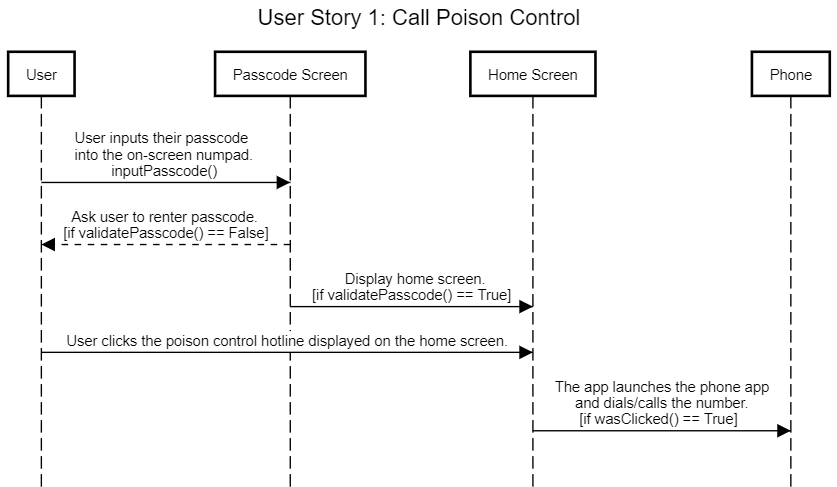
\includegraphics[scale=.45]{User_Story_1__Call_Poison_Control}~\cite{seqdia}
\newline
\newline
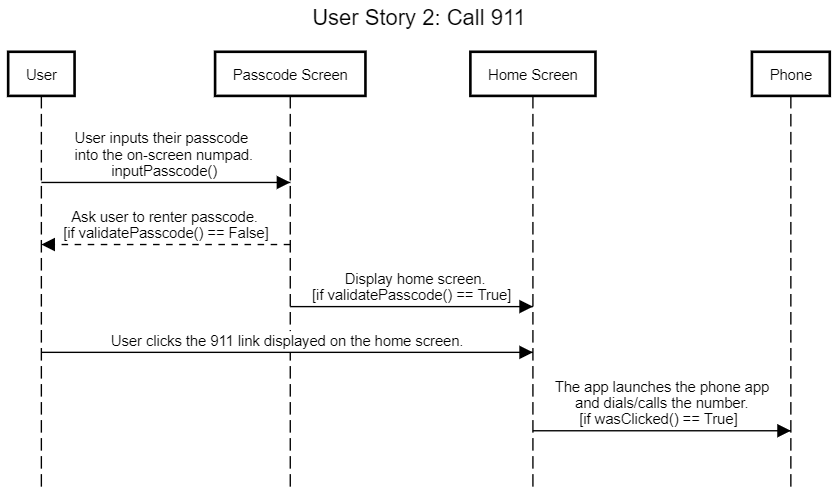
\includegraphics[scale=.45]{User_Story_2__Call_911}~\cite{seqdia}
\newline
\newline
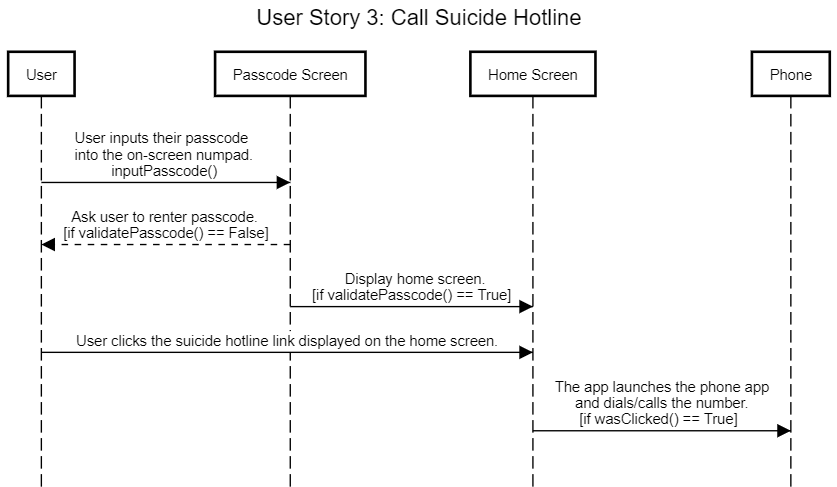
\includegraphics[scale=.45]{User_Story_3__Call_Suicide_Hotline}~\cite{seqdia}
\newline
\newline
\hspace*{-.5in}
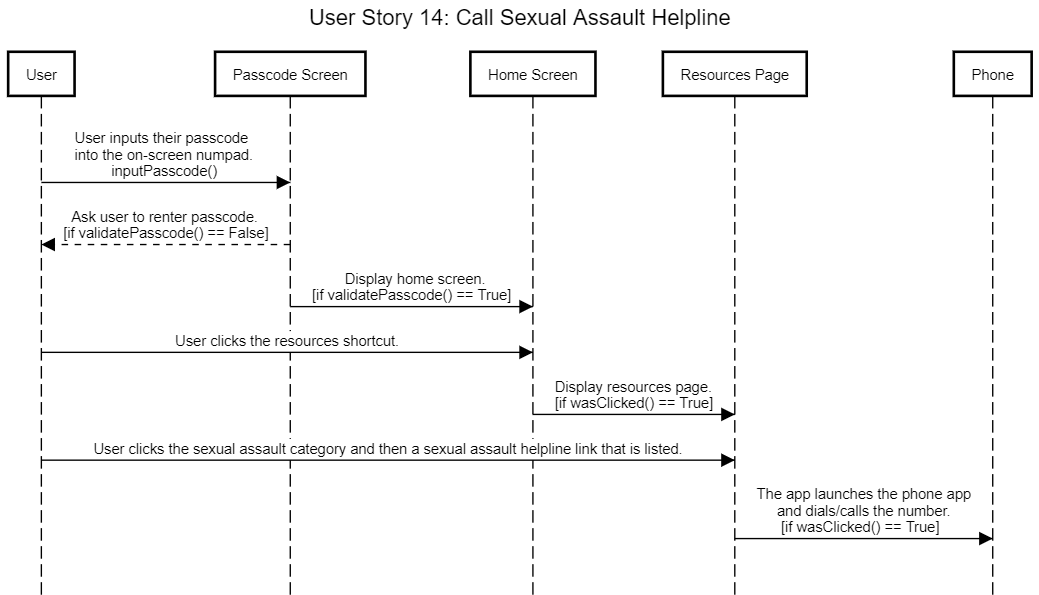
\includegraphics[scale=.45]{User_Story_14__Call_Sexual_Assault_Helpline}~\cite{seqdia}
\newline
\newline
\hspace*{-.5in}
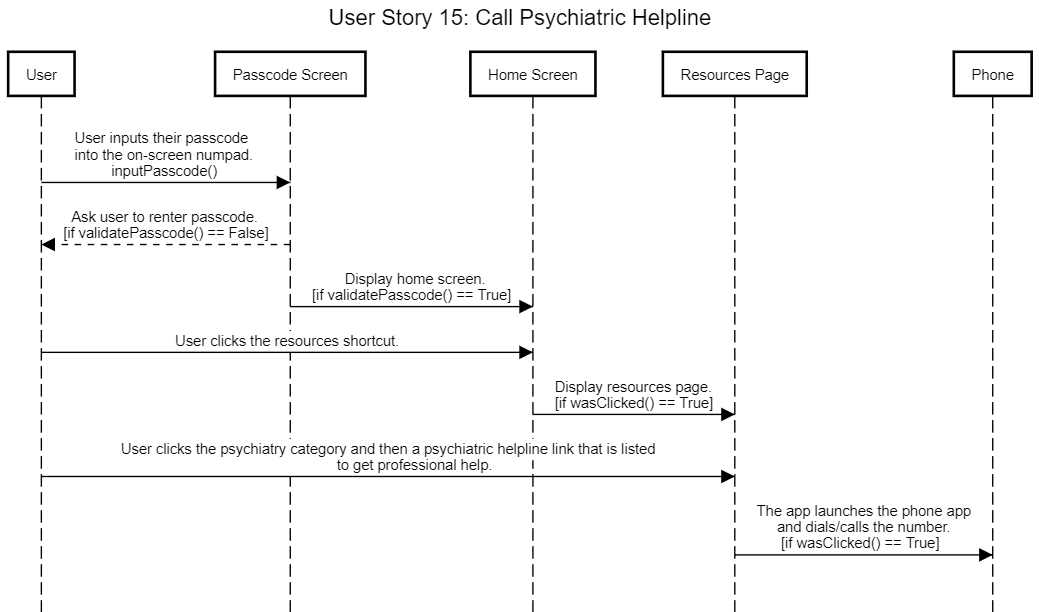
\includegraphics[scale=.45]{User_Story_15__Call_Psychiatric_Helpline}~\cite{seqdia}
\newline
\newline
\hspace*{-.5in}
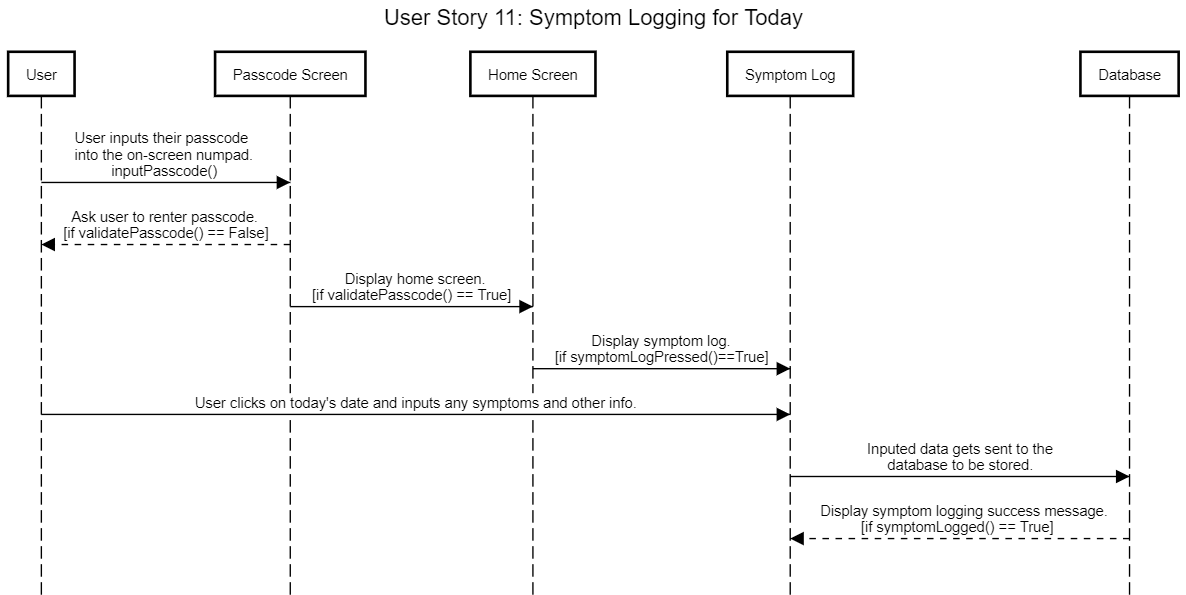
\includegraphics[scale=.4]{User_Story_11__Symptom_Logging_for_Today}~\cite{seqdia}
\newline
\newline
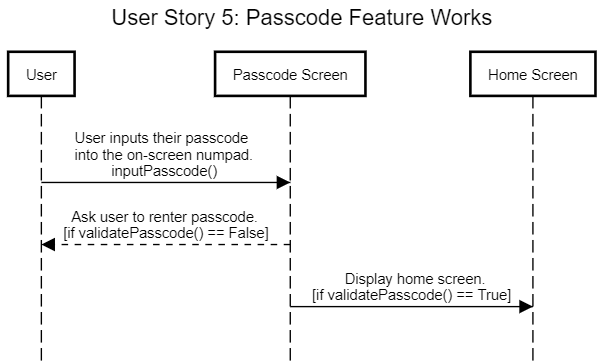
\includegraphics[scale=.66]{User_Story_5__Passcode_Feature_Works}~\cite{seqdia}

\newpage
\section{Stories Due Next Week}
\textbf{Story: Calling}
\newline
Assigned team members: Megan
\newline
Due Date: 3/5/2018
\newline
\newline
Megan will be implementing the calling functionality until next week (3/5/2018). She will be working on setting up the app so that, when given the necessary permission, it can access the phones calling app and dial/call the numbers that are clicked by the user within the WellLiv app. She will then commit the changes to github by next week.
\newline
\newline
\textbf{Story: Symptom log (current)}
\newline
Assigned team members: Katherine
\newline
Due Date: 3/5/2018
\newline
\newline
Katherine will be implementing the symptom log until next week (3/5/2018). She will work on the log so that the user can add their symptoms for the current day. She will then commit the changes to github by next week.
\newline
\newline
\textbf{Story: Passcode}
\newline
Assigned team members: Sarahi
\newline
Due Date: 3/5/2018
\newline
\newline
Sarahi will be implementing the passcode functionality until next week (3/5/2018). She will work on functions for determining whether the entered passcode is correct or not and will implement error handling. She will then commit the changes to github by next week.
\newline
\newline
\textbf{Stories due the week after the next:}
\begin{itemize}
\item Logging(previous)
\item Looking at symptoms
\item Hard coded information
\item Links to external sites
\end{itemize}
\newpage
\section{Meeting Report}
\underline{Fifth meeting:} 2/22 in person at 12:30pm-1:30pm
\begin{itemize}
\item Members present: Sarahi Pelayo, Katherine Jeffrey, Jonathan Rohr
\item Discussed: Design of the home button to the logo and user stories.
\item Progress: Sarahi and Jonathan designed the logo, Jonathan created it then added it to the code on github. Sarahi made a list of stories. Katherine added a menu to the log symptoms which has three categories: mental, physical, and mood. New code was merged together. Some tasks were outlined based on corresponding stories.
\item Plans: Explain all the progress to the rest of the team at a the next meeting today. Create tasks based on the stories. Estimate effort and difficulty of implementation. Assign tasks or spikes to subgroups.
\item Customers were willing and able to meet.
\end{itemize}
\noindent
\underline{Sixth meeting:} 2/22 after class in person, 5:50pm-6:30pm
\begin{itemize}
\item Members present: Sarahi Pelayo, Katherine Jeffrey, Jonathan Rohr, Johnathan Lee, Megan Bigelow
\item Discussed: Progress and what happened in the earlier meeting. How to estimate effort and rank difficulty. 
\item Progress: We decided when which tasks will get done. Ranked difficulties, and estimated effort. Assigned the tasks to individuals/subgroups.
\item Plans: Finish tasks, and either make UML diagrams or spikes.
\item Customers were willing and able to meet.
\end{itemize}
\textbf{Next Week}
\begin{itemize}
\item Tackle tasks in subteams and add functionality
\end{itemize}
\newpage

\bibliography{myref}
\bibliographystyle{ieeetr}
\textbf{GitHub Repo:} \url{https://github.com/Rohrj/CS361-001-W2018/tree/Assignment-5/projects/rohrj}

\end{document}